% Options for packages loaded elsewhere
\PassOptionsToPackage{unicode}{hyperref}
\PassOptionsToPackage{hyphens}{url}
%
\documentclass[
]{article}
\usepackage{amsmath,amssymb}
\usepackage{lmodern}
\usepackage{iftex}
\ifPDFTeX
  \usepackage[T1]{fontenc}
  \usepackage[utf8]{inputenc}
  \usepackage{textcomp} % provide euro and other symbols
\else % if luatex or xetex
  \usepackage{unicode-math}
  \defaultfontfeatures{Scale=MatchLowercase}
  \defaultfontfeatures[\rmfamily]{Ligatures=TeX,Scale=1}
\fi
% Use upquote if available, for straight quotes in verbatim environments
\IfFileExists{upquote.sty}{\usepackage{upquote}}{}
\IfFileExists{microtype.sty}{% use microtype if available
  \usepackage[]{microtype}
  \UseMicrotypeSet[protrusion]{basicmath} % disable protrusion for tt fonts
}{}
\makeatletter
\@ifundefined{KOMAClassName}{% if non-KOMA class
  \IfFileExists{parskip.sty}{%
    \usepackage{parskip}
  }{% else
    \setlength{\parindent}{0pt}
    \setlength{\parskip}{6pt plus 2pt minus 1pt}}
}{% if KOMA class
  \KOMAoptions{parskip=half}}
\makeatother
\usepackage{xcolor}
\IfFileExists{xurl.sty}{\usepackage{xurl}}{} % add URL line breaks if available
\IfFileExists{bookmark.sty}{\usepackage{bookmark}}{\usepackage{hyperref}}
\hypersetup{
  hidelinks,
  pdfcreator={LaTeX via pandoc}}
\urlstyle{same} % disable monospaced font for URLs
\usepackage{graphicx}
\usepackage{listings}


\makeatletter
\def\maxwidth{\ifdim\Gin@nat@width>\linewidth\linewidth\else\Gin@nat@width\fi}
\def\maxheight{\ifdim\Gin@nat@height>\textheight\textheight\else\Gin@nat@height\fi}
\makeatother
% Scale images if necessary, so that they will not overflow the page
% margins by default, and it is still possible to overwrite the defaults
% using explicit options in \includegraphics[width, height, ...]{}
\setkeys{Gin}{width=\maxwidth,height=\maxheight,keepaspectratio}
% Set default figure placement to htbp
\makeatletter
\def\fps@figure{htbp}
\makeatother
\setlength{\emergencystretch}{3em} % prevent overfull lines
\providecommand{\tightlist}{%
  \setlength{\itemsep}{0pt}\setlength{\parskip}{0pt}}
\setcounter{secnumdepth}{-\maxdimen} % remove section numbering
\ifLuaTeX
  \usepackage{selnolig}  % disable illegal ligatures
\fi

\author{}
\date{}

\begin{document}

\textbf{REMOTE ACCESS -TUTORIAL}

\textbf{MobaXterm, Public Key Authentication and .bashrc Settings}

\textbf{MobaXterm CLIENT -TUTORIAL}

\begin{enumerate}
\def\labelenumi{\Alph{enumi}.}
\item
  \textbf{MobaXterm Installation}
\end{enumerate}

\begin{enumerate}
\def\labelenumi{\arabic{enumi}.}
\item
  Download MobaXterm from
  \url{https://mobaxterm.mobatek.net/download.html}
\item
  Install it with default settings.
\end{enumerate}

\begin{enumerate}
\def\labelenumi{\Alph{enumi}.}
\setcounter{enumi}{1}
\item
  \textbf{MobaXterm Configuration}
\end{enumerate}

\begin{enumerate}
\def\labelenumi{\arabic{enumi}.}
\setcounter{enumi}{2}
\item
  Click on "Sessions" and then on "SSH".
\end{enumerate}

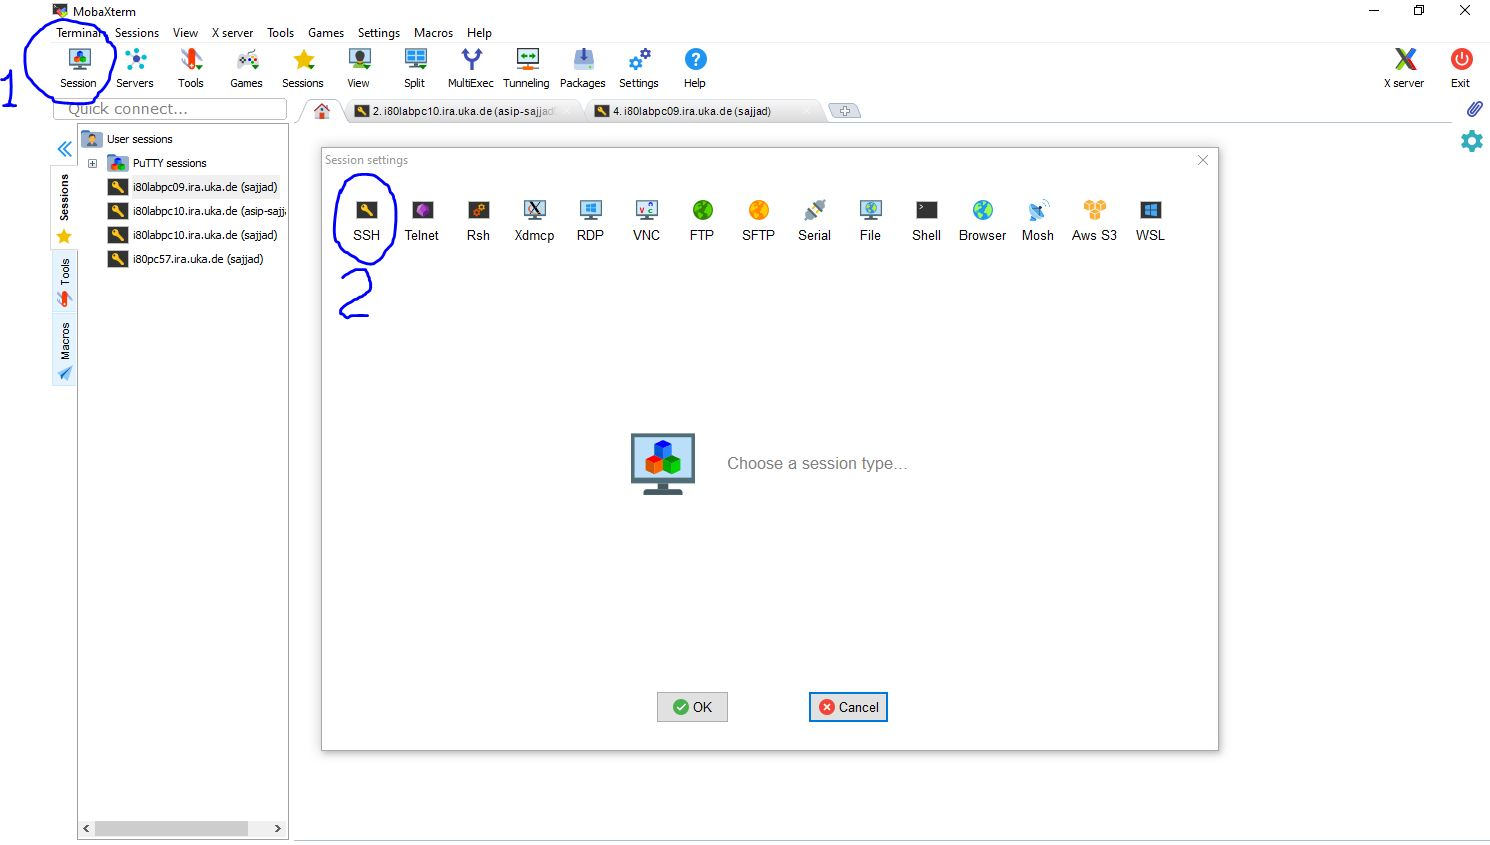
\includegraphics[width=5.73515in,height=3.25226in]{images/media/image1.JPG}

Figure : SSH Session

\begin{enumerate}
\def\labelenumi{\arabic{enumi}.}
\setcounter{enumi}{3}
\item
  In the new windows "Session settings", enter \textbf{Remote host} as
  ``\emph{i80labpcXX.ira.uka.de}'', tick the box "\textbf{Specify user
  name}" and then enter your user name as ``\emph{asip-abcdnn}''.
\end{enumerate}

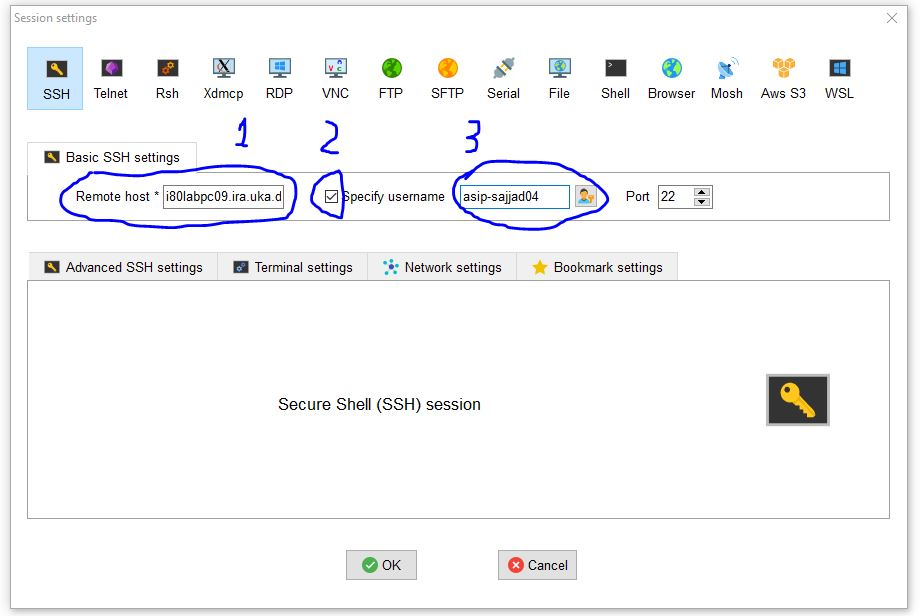
\includegraphics[width=5.53861in,height=3.70864in]{images/media/image2.JPG}

Figure : Session Settings

\begin{enumerate}
\def\labelenumi{\arabic{enumi}.}
\setcounter{enumi}{4}
\item
  Press OK. It will ask for the user password.
\item
  Enter your password and press Enter.
\end{enumerate}

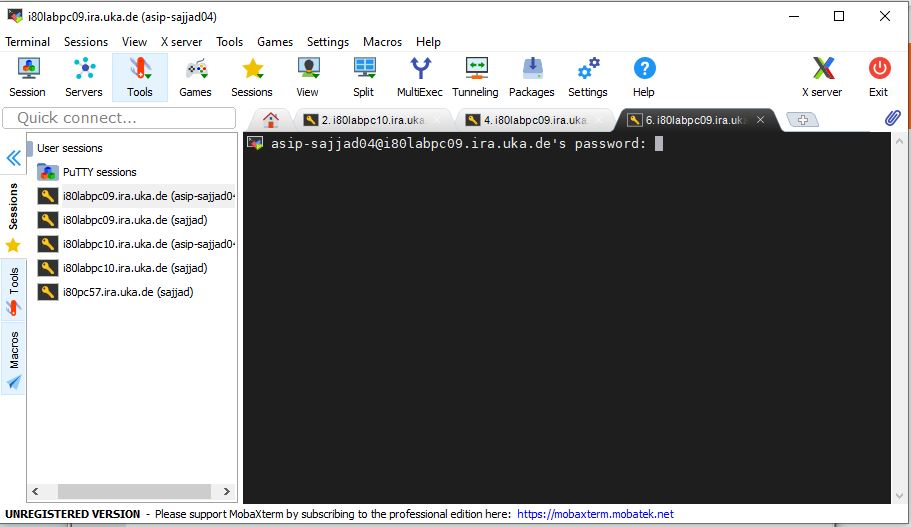
\includegraphics[width=5.67963in,height=3.28535in]{images/media/image3.JPG}

Figure : Logging in and Requiring Password

\begin{enumerate}
\def\labelenumi{\arabic{enumi}.}
\setcounter{enumi}{6}
\item
  You are now logged into the lab PC using MobaXterm.
\end{enumerate}

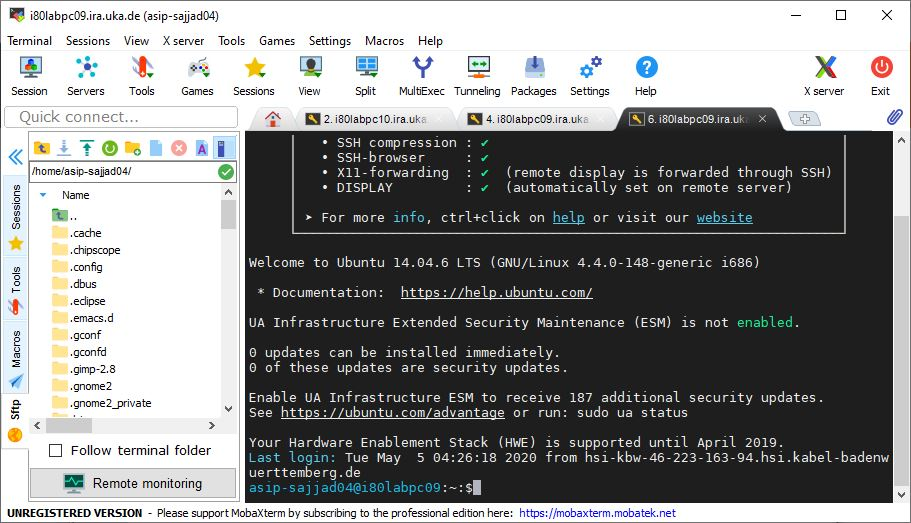
\includegraphics[width=5.70556in,height=3.27527in]{images/media/image4.JPG}

Figure : Logged into Remote PC

\begin{enumerate}
\def\labelenumi{\Alph{enumi}.}
\setcounter{enumi}{2}
\item
  \textbf{Recommended Practice.}
\end{enumerate}

\begin{enumerate}
\def\labelenumi{\arabic{enumi}.}
\setcounter{enumi}{7}
\item
  It is \textbf{recommended} to log into \textbf{i80pc57} as this PC
  contains the ASIPmeister software. Try to perform lab on this PC. Use
  \textbf{i80labpc10} when you need to implement your applications on
  FPGA.
\item
  To repeatedly login to some PC and avoid password, use DSA-keys and
  copy to desired PC.
\item
  Type "\textbf{ssh-keygen -t dsa}" and press Enter. Leave the default
  options. Leave the password empty.
\end{enumerate}
\begin{lstlisting}
asip-sajjad04@i80labpc09:~:$ssh-keygen -t dsa
Generating public/private dsa key pair.
Enter file in which to save the key (/home/asip-sajjad04/.ssh/id_dsa):
/home/asip-sajjad04/.ssh/id_dsa already exists.
Overwrite (y/n)? y
Enter passphrase (empty for no passphrase):
Enter same passphrase again:
Your identification has been saved in /home/asip-sajjad04/.ssh/id_dsa.
Your public key has been saved in /home/asip-sajjad04/.ssh/id_dsa.pub.
The key fingerprint is:
af:c3:84:62:4e:f4:e6:5e:cb:d1:03:19:ff:63:a9:ad asip-sajjad04@i80labpc09
The key's randomart image is:
+--[ DSA 1024]----+
|                 |
|                 |
|        .        |
|    .    +       |
|   . . .S .      |
|    + + .+ . .   |
|   + + oo + =    |
|    . .oo+ = .   |
|     .. +.E..    |
+-----------------+
\end{lstlisting}
\begin{lstlisting}

asip-sajjad04@i80labpc09:\textasciitilde:\$ssh-keygen -t dsa

Generating public/private dsa key pair.

Enter file in which to save the key (/home/asip-sajjad04/.ssh/id\_dsa):

/home/asip-sajjad04/.ssh/id\_dsa already exists.

Overwrite (y/n)? y

Enter passphrase (empty for no passphrase):

Enter same passphrase again:

Your identification has been saved in /home/asip-sajjad04/.ssh/id\_dsa.

Your public key has been saved in /home/asip-sajjad04/.ssh/id\_dsa.pub.

The key fingerprint is:

af:c3:84:62:4e:f4:e6:5e:cb:d1:03:19:ff:63:a9:ad asip-sajjad04@i80labpc09

The key's randomart image is:

+-\/-{[} DSA 1024{]}-\/-\/-\/-+

\textbar{} \textbar{}

\textbar{} \textbar{}

\textbar{} . \textbar{}

\textbar{} . + \textbar{}

\textbar{} . . .S . \textbar{}

\textbar{} + + .+ . . \textbar{}

\textbar{} + + oo + = \textbar{}

\textbar{} . .oo+ = . \textbar{}

\textbar{} .. +.E.. \textbar{}

+-\/-\/-\/-\/-\/-\/-\/-\/-\/-\/-\/-\/-\/-\/-\/-\/-+
\end{lstlisting}
\begin{enumerate}
\def\labelenumi{\arabic{enumi}.}
\setcounter{enumi}{10}
\item
  Then copy this generated DSA-key to desired PC by type following
  command and enter your password.
\end{enumerate}

asip-sajjad04@i80labpc09:\textasciitilde:\$ssh-copy-id -i
\textasciitilde/.ssh/id\_dsa.pub asip-sajjad04@i80pc57

/usr/bin/ssh-copy-id: INFO: attempting to log in with the new key(s), to
filter out any that are already installed

/usr/bin/ssh-copy-id: INFO: 1 key(s) remain to be installed -\/- if you
are prompted now it is to install the new keys

asip-sajjad04@i80pc57's password:

Number of key(s) added: 1

Now try logging into the machine, with: "ssh 'asip-sajjad04@i80pc57'"

and check to make sure that only the key(s) you wanted were added.

\begin{enumerate}
\def\labelenumi{\arabic{enumi}.}
\setcounter{enumi}{11}
\item
  Now log into i80pc57 using ``ssh -X'' it will ask for the password.
\end{enumerate}

asip-sajjad04@i80labpc09:\textasciitilde:\$ssh -X i80pc57

Last login: Wed May 6 05:11:07 2020 from i80labpc09.irf.uni-karlsruhe.de

asip-sajjad04@i80pc57:\textasciitilde:\$

\begin{enumerate}
\def\labelenumi{\Alph{enumi}.}
\setcounter{enumi}{3}
\item
  \textbf{Setting up .bashrc.user}
\end{enumerate}

\begin{enumerate}
\def\labelenumi{\arabic{enumi}.}
\setcounter{enumi}{12}
\item
  Whenever you are logged into any PC, this file is executed at the
  login. Please set different variables in this file carefully. Usually
  the following variables should be like this:
\end{enumerate}

asip-sajjad04@i80pc57:\textasciitilde:\$cat .bashrc.user

export ASIPS\_LICENSE=29000@i80asip.ira.uka.de

export PATH=/AM/ASIPmeister/bin:\$PATH

export ASIP\_APDEV\_SRCROOT=/home/asip00/epp/AM\_tools

export PATH=/usr/java/jre1.6.0\_45/bin:\$PATH

export ASIPmeister\_Home=/AM/ASIPmeister

export ASIPmeister\_HOME=/AM/ASIPmeister

. /home/adm/modelsim\_66d.setup

. /home/adm/xilinx\_13.2\_32bit.setup

asip-sajjad04@i80pc57:\textasciitilde:\$

\end{document}
